\documentclass[12pt]{article}
\usepackage{HomeWorkTemplate}
\usepackage{circuitikz}
\usepackage{tikz}
\usepackage{float}
\usepackage{amsmath}
\usepackage{xepersian}
\usetikzlibrary{arrows,automata}
\usetikzlibrary{circuits.logic.US}
\settextfont{XB Niloofar}
\newcounter{problemcounter}
\newcounter{subproblemcounter}
\newcommand{\E}{\mathbb{E}}
\linespread{1.2}
\setcounter{problemcounter}{1}
\setcounter{subproblemcounter}{1}
\newcommand{\grade}[1]{\textbf{(#1 نمره)}}
\newcommand{\problem}[1]
{
\subsection*{
مسأله‌ی
\arabic{problemcounter} 
\stepcounter{problemcounter}
\setcounter{subproblemcounter}{1}
#1
}
}
\newcommand{\subproblem}{
\textbf{\harfi{subproblemcounter})}\stepcounter{subproblemcounter}
}
\newcommand{\n}{

\null

}
\begin{document}
\handout
{نظریه‌ی زبان‌ها و اتوماتا}
{}
{علیرضا توفیقی محمدی}
{سری ۳}
{شماره‌دانشجویی: 96100363}

\problem{}
\subproblem{}
\begin{definition}
به زبانی مثل $A$،
$(x, y)$
معتدل گوییم هرگاه هر رشته مثل $w \in A$ دارای شرایط زیر باشد:
\begin{enumerate}
	\item 
	$w$
	متشکل از $x$ و $y$ باشد.
	\item
	تعداد $x$‌ها و $y$‌ها در $w$ برابر باشند.
	\item
	به ازای هر پیشوند از $w$ تعداد $x$ها بیشتر یا مساوی تعداد $y$ ها باشد.
\end{enumerate}
\end{definition}

از مطالب داخل جزوه و کلاس می‌دانیم زبان‌های $(x,y)$ متعادل مستقل از متن اند و گرامری به شکل زیر دارند:
$$
S \rightarrow xSy|\epsilon|SS
$$

\begin{definition}
	به رشته‌ی $w$ جذاب گوییم هرگاه $n_0(w) = n_1(w)$.
\end{definition}
فرض کنید 
$w$
رشته‌ای جذاب باشد و $n$ بزرگترین عددی باشد که
$w = w_1 w_2 ... w_n$
باشد و $w_i$ها جذاب باشند.

چون $n$ بزگترین عدد است، $w_i$‌ها باید $(0, 1)$ معتدل یا $(1, 0)$ معتدل باشند. (زیرا در غیر اینصورت $l$ و $r$‌ای موجود است که تعداد ۱‌ها در پیشوند به طول یکی از $x$ و $y$  ۰‌ها بیشتر و در دیگری کمتر باشد و در نتیجه $x$ای بین $l$ و $r$ وجود دارد که تعداد ۰‌ها و یک‌ها در پیشوند به طول $x$ از $w_i$ برابر باشد و می‌توان $w_i$ را به دو رشته‌ی جذاب تبدیل کرد و $w$ را به $n+1$ رشته‌ی جذاب تقسیم کرد که تناقض است.)

پس هر $w$ که جذاب باشد به صورت 
$(l + r)^*$
که $l$ رشته‌ای $(0, 1)$ متعادل و $r$ رشته‌ای $(1, 0)$ متعادل است.

همچنین عمل بستار و جمع را با گرامر‌ها بلدیم و می‌توانیم زبان 
$L = \{w \in {0, 1}^* | n_0(w) = n_1(w)\}$
را به شکل زیر بسازیم:
$$S \rightarrow AS|BS|\epsilon$$
$$A \rightarrow 0A1|AA|\epsilon$$
$$B \rightarrow 1B0|BB|\epsilon$$

\subproblem{}
با توجه به توضیحات بند الف، می‌توان به همین نحو و با کمک ماشین پشته‌ای نیز این زبان را ساخت:

$$\Gamma = \{Z_0, X\} , F = \{q_0\}$$

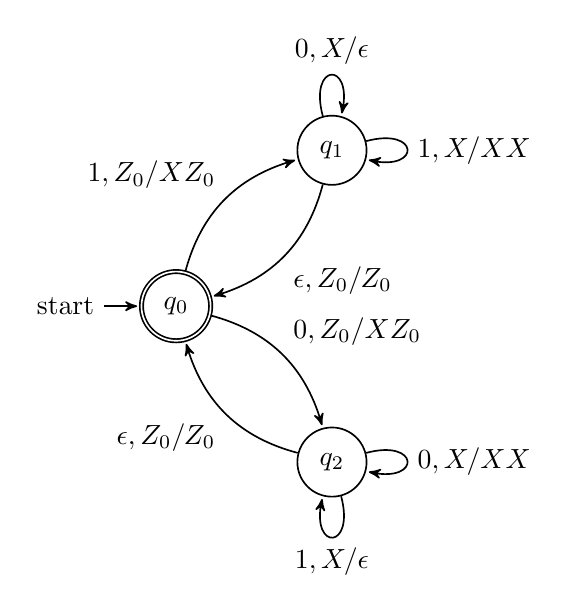
\begin{tikzpicture}[->,>=stealth',shorten >=1pt,auto,node distance=2.8cm,semithick]

\node[initial,state,accepting] (0)                {$q_0$};
\node[state]         (1) [above right of=0] {$q_1$};
\node[state]	     (2)  [below right of=0] {$q_2$};

\path
(0)  edge [bend left] node {$1,Z_0 / XZ_0$} (1)
(1)  edge [bend left] node {$\epsilon,Z_0 / Z_0$} (0)
(0)  edge [bend left] node {$0,Z_0 / XZ_0$} (2)
(2)  edge [bend left] node {$\epsilon,Z_0 / Z_0$} (0)

(1) edge [loop right] node {$1,X / XX$} (1)
(1) edge [loop above] node {$0,X / \epsilon$} (1)


(2) edge [loop right] node {$0,X / XX$} (1)
(2) edge [loop below] node {$1,X / \epsilon$} (1)
;
\end{tikzpicture}

که حالت بالا راست برای $(1,0)$ متعادل‌ها و حالت پایین برای $(0, 1)$ متعادل هاست.
به سادگی با کمک استقرا روی تعداد حداکثر $n$ای که $w$ را می‌توان به $n$ رشته‌ی جذاب افراز کرد مسئله را حل کرد و همچنین استقرا روی تعداد دفعه‌هایی که $PDA$ به حالت $q_0$ می‌رسد ثابت کرد ماشین پشته‌ای ساخته شده درست کار می‌کند.

\problem{}
\subproblem{}
برهان خلف می‌زنیم، فرض کنید $DPDA$ای مانند
$D = (Q, \{0, 1\}, \Gamma, \delta, q_0, Z_0, F)$
وجود دارد که 
$$L(D) = \{0^n1^n \cup 0^n1^{2n} | n \geq 1\}$$
(بدون خدشه به کلیت مسئله فرض می‌کنیم پشته‌ی این ماشین هیچ‌گاه خالی نمی‌شود. (با ساختن یک حالت اولیه جدید که $\epsilon$ از رشته و $Z_0$ از پشته را می‌خواند و به حالت اولیه قبل رفته و $Z_0\#$ که $\#$ یک حرف جدید است را به پشته اضافه می‌کند.))
حال با کمک $D$ یک ماشین پشته‌ای دیگر مثل $D'$ می‌سازیم که 
$L(D') = \{0^n 1^n 2^n | n \geq 1\}$
باشد و به تناقض می‌رسیم.

برای این کار 
$$D' = (Q', \{0, 1, 2\}, \Gamma, \delta', (0, q_0), Z_0, F')$$
در نظر بگیرید که
$$
Q' = \{(x, q) | x \in \{0, 1\}, q \in Q\}
$$
$$
F' = \{(1, q) | q \in F \}
$$
$$
\forall X \in \Gamma, a \in \Sigma \cup \{\epsilon\}, q \in Q - F: \delta'((0, q), a, X) = \{((0, p), \gamma) | (p, \gamma) \in \delta(q, a, X)\}
$$
$$
\forall X \in \Gamma, a \in \Sigma, q \in F: \delta'((0, q), a, X) = \{((0, p), \gamma) | (p, \gamma) \in \delta(q, a, X)\}
$$
$$
\forall X \in \Gamma, q \in F: \delta'((0, q), \epsilon, X) = \{((0, p), \gamma) | (p, \gamma) \in \delta(q,\epsilon, X)\} \cup \{((1,q), X)\}
$$
$$
\forall X \in \Gamma, q \in Q: \delta'((2, q), \epsilon, X) = \{((2, p), \gamma) | (p, \gamma) \in \delta(q, \epsilon, X)\}
$$
$$
\forall X \in \Gamma, q \in Q: \delta'((2, q), 0, X) = \{((2, p), \gamma) | (p, \gamma) \in \delta(q, 0, X)\}
$$
$$
\forall X \in \Gamma, q \in Q: \delta'((2, q), 2, X) = \{((2, p), \gamma) | (p, \gamma) \in \delta(q, 1, X)\}
$$
(در واقع یک کپی از ماشین پشته‌ای ساختیم و در ماشین پشته‌ای جدید به جای یک، دو گذاشته و حالت‌های نهایی ماشین اول را با خواندن $\epsilon$ به حالت نهایی متناظر در ماشین دوم وصل می‌کنیم و حالت‌های نهایی را حالت‌های نهایی کپی‌شده می‌گذاریم.)

به سادگی می‌توان دید زبان ماشین دوم به صورت
$L' = \{w | w = 0^n1^n \lor w = 0^n1^{2n} \lor w= 0^n1^n2^n , n \geq 1 \}$
است.

حال چون $L'$ توسط یک ماشین پشته‌ای پذیرفته شده است، لم تزریق برای آن برقرار است و عددی مثل $n$  وجود دارد که هررشته مثل $w$ که $w \in L', |w| \geq n$ باشد را می‌توان به شکل شرایط لم تزریق نوشت، این رشته را 
$0^{2n}1^{2n}2^{2n} = w$
 در نظر بگیرید، طبق لم تزریق داریم:
\begin{enumerate}
	\item $w = abcde$
	\item $bcd \leq n$
	\item $|bd| \geq 1$
	\item $\forall i ab^icd^ie \in L'$
\end{enumerate}
که چون 
$w=0^{2n}1^{2n}2^{2n}$
 است، $bcd$ یا ۰ را شامل نمی‌شود یا ۱ را شامل نمی‌شود، در نتیجه رشته‌ی
$ace$
دارای تعداد نامساوی از ۰ و ۱ و ۲ است و از هر کدام حداقل یکی دارد، پس نمی‌تواند در $L'$ باشد که تناقض است. پس فرض خلف باطل و حکم ثابت است.

\problem{} % 3

\problem{} % 4

\problem{} % 5
\subproblem{}
$$
S \rightarrow a | aSa | aSb | bSa | bSb
$$
اگر زبان گرامر بالا را $G$ و زبان همه‌ی کلمات به طول فرد که حرف وسط آن‌ها $a$ است را $L$ در نظر بگیریم، باید ثابت کنیم 
$$
L = G \iff L \subseteq G \land G \subseteq L
$$

\textbf{اثبات $L \subseteq G$}\\
فرض کنید $w \in L$ باشد، با استقرا روی طول $w$ ثابت می‌کنیم $w \in G$.

پایه:‌ اگر $|w| = 1$ آنگاه $w=a$ که واضح است در $G$ است.

حال فرض کنید برای همه‌ی $w$‌هایی که $|w| < n$ است، $w$ توسط متغیر $S$ ساخته شود.

حال $w$ای که $|w| = n$ در نظر بگیرید و فرض کنید
$w = w_1 w_2 ... w_n$
و $n > 2$، حال رشته‌ی 
$w' = w_2 w_3 ... w_{n-1}$
را در نظر بگیرید، $w'$ نیز رشته‌ای به طول فرد است که وسط آن حرف $a$ است، پس طبق فرض استقرا توسط $S$ تولید می‌شود.

حال چون در قواعد تولید به ازای هر $x, y \in \Sigma$، قاعده‌ی $S \rightarrow xSy$ را در قواعد تولید داریم، پس با کمک قاعده‌ی $S \rightarrow w_1Sw_n$ و تولید شدن $w'$ از $S$ طبق استنتاج بازگشتی $S$ رشته‌ی $w = w_1w'w_n$ را نیز تولید می‌کند و مسئله حل شد.

\textbf{اثبات $G \subseteq L$}\\
برای اثبات فرض کنید رشته‌ی $w$ از روی متغیر $S$ استنتاج شده‌باشد، با استقرا روی تعداد مراحل استنتاج ثابت می‌کنیم $w \in L$.

پایه:‌ اگر تعداد مراحل استنتاج یک باشد در این صورت فقط رشته‌ی $a$ را می‌توانیم بسازیم که در زبان است.

حال فرض کنید هر رشته‌ای با حداکثر $k$ مرحله استنتاج ساخته شود در $L$ باشد، حال رشته‌ی $w$ را در نظر بگیرید که با $k+1$ مرحله استنتاج ساخته شده‌باشد، این رشته در آخرین مرحله‌ی استنتاج بازگشتی از یکی از قوانین تولید استفاده کرده، چون قوانین تولیدی که سمت راستشان متغیر است، همه دارای تک متغیر $S$ اند و این $S$ باید با حداکثر $k$ مرحله استنتاج ساخته شده‌باشد، طبق فرض استقرا رشته‌ای با طول فرد است که حرف وسط آن $a$ است، حال با توجه به قواعد تولید دوطرف این $S$ یک حرف قرار می‌دهیم که رشته‌ی جدید نیز در $L$ است، پس گام استقرا نیز ثابت شد.

پس حکم ثابت شد و $L = G$.

\subproblem{}
$$
S \rightarrow a|baAa|bBb
A \rightarrow a|aAa|aAb|bAa|bAb
B \rightarrow b|aBa|aBb|bBa|bBb 
$$

طبق توضیحات بالا و با توجه به مشابه بودن گرامر با گرامر قسمت الف، زبان تولید شده از متغیر $A$ تمام رشته‌های فرد حرفی اند که حرف وسط آن‌ها $a$ است و زبان تولید شده از متغیر $B$ تمام رشته‌های فرد حرفی‌اند که حرف وسط آن‌ها $b$ است.

حال یک رشته ۲ حالت دارد، حرف وسط و اول و آخر آن $a$ باشد که در این صورت به شکل $aAa$ یا $a$ است و یا حرف وسط، اول و آخر آن $b$ است که به شکل $bBb$ یا $b$ است که متغیر $S$ تنها به این دو حالت را می‌سازد پس گرامر تولید‌شده درست است.
\problem{} % 6

\problem{}
همه‌ی متغیر‌ها پوچ سازند پس:
$$
S \rightarrow A | B | C | AB | AC | BC | ABC
$$$$
A \rightarrow B | A  | BA | C | BC | a
$$$$
B \rightarrow A | C | AB | B | CB | b
$$$$
C \rightarrow B | C | BC | A | AB | c
$$

\problem{} % 8
ابتدا قواعد تولید $\epsilon$ را از گرامر حذف می‌کنیم:
$$
S \rightarrow S(S) | (S) | S() | ()
$$
حال متغیر‌های غیر مولد و غیرقابل درسترس را حذف می‌کنیم که متغیری نداریم.
\\
سپس با تعریف متغیر‌های جدید گرامر را به فرم نرمال تبدیل می‌کنیم:
$$
S \rightarrow SX | AY | SZ | AB
$$$$
X \rightarrow AY
$$$$
Y \rightarrow SB
$$$$
A \rightarrow (
$$$$
B \rightarrow )
$$

\problem{} % 9
\subproblem{} %A

(در ماشین کشیده شده $c$ به معنی یک حرف پشته‌ی دلخواه است.)

$$\Gamma = \{Z_0, X, Y\} , F = \{q_1\}$$

\begin{tikzpicture}[->,>=stealth',shorten >=1pt,auto,node distance=2.8cm,semithick]

\node[initial,state] (0)                {$q_0$};
\node[state,accepting]         (1) [right of=0] {$q_1$};

\path
(0)  edge [loop above] node {$(,c / Xc$ و $\{, c / Yc$ و
$), X / \epsilon$ و $\}, Y, \epsilon$
 } (0)
(0) edge [] node {$\epsilon, Z_0/ \epsilon$} (1)
;
\end{tikzpicture}

\subproblem{} % B

\problem{} % 10
چون تعداد دنباله‌های به طول حداکثر $k$ از حروف $\Gamma$ متناهی است پس یک 
\enfa
می‌سازیم که حالت‌هایش دوتایی از حالت‌های ماشین پشته‌ای و دنباله‌ای به طول حداکثر $k$ از $\Gamma$ باشد.
یعنی اگر 
$P = (\Sigma, \Gamma, Q, q_0, Z_0, \delta, F)$
ماشین پشته‌ای باشد یک \enfa مثل $E$ به شکل زیر ارائه می‌دهیم:
$$
E = (\Sigma, Q', q_0', \delta', F')
$$
$$
Q' = \{(q, y) | q \in Q \land y = X_1...X_l , l \leq k, X_i \in \Gamma\}
$$
$$
q_0' = (q_0, Z_0)
$$
$$
\delta'((q, X_1...X_l), x) = \left\{(p, X_1...X_{l-1}\gamma) | x \in \Sigma \cup {\epsilon} \land p \in Q \land \gamma \in \Gamma^* \land (p, \gamma) \in \delta(q, x, X_l) \right\}
$$
$$
F' = \{(q, X_1...X_l) | q \in F \land X_i \in \Gamma \land l \leq k\}
$$

حال ادعا می‌کنیم $L(E) = L(P)$. که اثبات آن با توجه به فرض مسئله و ویژگی‌های اتوماتای ساخته‌شده نسبتا واضح است زیرا متناظر هر حالت و هر حالت از پشته یک حالت در \enfa داریم و حرکت‌های روی 
\lr{PDA}
 دقیقا متناظر با حرکت‌های روی \enfa است.
\problem{} % 11

\problem{} % 12
\subproblem{} % A
اگر زبان مستقل از متن باشد پس $n$ ای وجود دارد که برای هر رشته با طول بیشتریا مساوی $n$ در زبان، لم‌تزریق برقرار باشد.

حال $m = \max(n, 10)$ در نظر بگیرید و رشته‌ی 
$w = a^{2^m}$
در نظر بگیرید، چون 
$|w| \geq n$
پس 
$w = uvxyz$
است که 
$|uxy| \leq n$
و
$|uy| > 0$
و
$uxz$
نیز در زبان است.

از طرفی
$2^m > |uxz| \geq 2^m - n > 2^{m-1}$

پس نمی‌تواند در زبان باشد و این تناقض است.

پس فرض خلف باطل و زبان مستقل از متن نیست.

\subproblem{} % B
اگر زبان مستقل از متن باشد پس $n$ ای وجود دارد که برای هر رشته با طول بیشتریا مساوی $n$ در زبان، لم‌تزریق برقرار باشد.

حال رشته‌ی 
$w = a^{n}b^{2n}a^n$
در نظر بگیرید، چون 
$|w| \geq n$
پس 
$w = uvxyz$
است که 
$|uxy| \leq n$
و
$|uy| > 0$
و
$uxz$
نیز در زبان است.

چون تعداد $b$های وسط بیشتر از $n$ تاست، $uxy$ رشته‌های $a$های چپ یا راست یا شامل نمی‌شود. پس رشته‌ی $uxz$ یا دارای تعداد $a$های نابرابر در دو طرف یا $b$های نابرابر با تعداد کل $a$ هاست، پس در زبان تیست.

پس فرض خلف باطل و زبان مستقل از متن نیست.


\subproblem{} % C
اگر زبان مستقل از متن باشد پس $n$ ای وجود دارد که برای هر رشته با طول بیشتریا مساوی $n$ در زبان، لم‌تزریق برقرار باشد.

حال رشته‌ی 
$w = a^{n}b^{n-1}c^{n}$
در نظر بگیرید، چون 
$|w| \geq n$
پس 
$w = uvxyz$
است که 
$|uxy| \leq n$
و
$|uy| > 0$
و
$uxz$
نیز در زبان است.

چون تعداد $b$های وسط کمتر از $n$ تاست، $uy$ حتما شامل $a$ یا $c$ است، از طرفی نمی‌تواند شامل هردو باشد، پس در رشته‌ی $uxz$ دقیقا تعداد یکی از $a$ و $c$ کمتر از $n$ است و دیگری برابر با $n$ است که در نتیجه $uxz$ در زبان نیست که این تناقض است.

پس فرض خلف باطل و زبان مستقل از متن نیست.
\problem{} % 13
برای اثبات از تمرین سری یک زیر به عنوان یک لم بدون اثبات استفاده می‌کنیم. (اثبات آن را در سری یک نوشتم و از تکرار پرهیز می‌کنم:)
\begin{lemma}
اگر
$L \subseteq {a}^*$
برابر با اجتماع متناهی تصاعد حسابی باشد، آن‌گاه $L$ منظم است.
\end{lemma}

با توجه به 
با توجه به لم تنها کافی است ثابت کنیم $L$ شامل متناهی تصاعد حسابی است، برای اینکار از لم تزریق استفاده می‌کنیم فرض کنید $n$ عدد لم تزریق باشد، فرض کنید رشته‌ی $w$ به طول $r$ عضو $L$ باشد که $r \geq n$ در این صورت $w = uvxyz$ است ک همه‌ی رشته‌های به شکل 
$uv^ixy^iz$
نیز عضو $L$ اند، یعنی اگر طول $vy$ برابر با $p$ باشد، همه‌ي رشته‌ها به طول
$r-p + kp = r' + kp$
نیز عضو زبان اند.

به ازای هر رشته دوتایی $(r', p)$ را تشکیل داده و مجموعه‌ی همه‌ی این دوتایی‌ها را $S$ می‌نامیم و ثابت می‌کنیم این دوتایی‌ها تعداد متناهی دنباله را می‌سازند پس کل زبان از تعداد متناهی دنباله حسابی تشکیل شده‌است.

برای این‌‌کار اولا می‌دانیم 
$1 \leq p \leq n$.

حال به ازای $p$ای بین ۱ تا $n$ و عددی مثل $x$ بین ۰ تا $p-1$، مجموعه‌ی 
$$A = \{w | (w, p) \in S, w \mod p = x\}$$
را در نظر بگیرید.

اگر $A$ تهی نبود، طبق اصل خوش‌ترتیبی در اعداد طبیعی مینیمم دارد، تعریف کنید
$w_0 := \min(A)$.
ادعا می‌کنیم همه‌ی دنباله‌ها با دوتایی $(w, p)$ که $w \mod p = x$ است توسط دنباله‌ با دوتایی
$(w_0, p)$
ساخته می‌شود. اثبات ادعا نیز واضح است زیرا این دنباله شامل همه‌ی اعداد بزرگتر یا مساوی $w_0$ که باقی‌مانده‌ی آن‌ها بر $p$ برابر با $x$ است، هست و بقیه‌ی دنباله‌ها برابر با مه‌ی اعداد بزرگتر یا مساوی $w$ که باقی‌مانده‌ی آن‌ها بر $p$ برابر با $x$ است، هستند که در نتیجه زیرمجموعه‌ی دنباله‌ی اول اند.

پس با کمک حداقل $n^2$ دنباله توانتسیم کل دنباله‌های تولیدی با کمک رشته‌های با طول بزرگتر‌یا مساوی $n$ را تولید کنیم، همچنین هر رشته با طول کمتر از $n$ خود یک تصاعد حسابی یک عضوی است. پس با کمک حداثل 
$n^2 + n$
تصاعد حسابی می‌توانیم زبان $L$ را بسازیم، پس طبق لم $L$ منظم است.
\problem{} % 14

فرض کنید $PDA$ای مانند
$P = (Q, \Sigma, \Gamma, \delta, q_0, Z_0, F)$
وجود دارد که 
$L(D) = L$.
(بدون خدشه به کلیت مسئله فرض می‌کنیم پشته‌ی این ماشین هیچ‌گاه خالی نمی‌شود. (با ساختن یک حالت اولیه جدید که $\epsilon$ از رشته و $Z_0$ از پشته را می‌خواند و به حالت اولیه قبل رفته و $Z_0\#$ که $\#$ یک حرف جدید است را به پشته اضافه می‌کند.))
حال با کمک $P$ یک ماشین پشته‌ای دیگر مثل $P'$ می‌سازیم که زبان آن همه‌ی پیشوند‌های $L$ باشد.

برای این کار 
$$P' = (Q', \Sigma, \Gamma, \delta', (0, q_0), Z_0, F')$$
در نظر بگیرید که
$$
Q' = \{(x, q) | x \in \{0, 1\}, q \in Q\}
$$
$$
F' = \{(1, q) | q \in F \}
$$
$$
\forall q \in Q, w \in \Sigma, X \in \Gamma: \delta'((0,q), w, X) = \{((0,q), Y) | (q, Y) \in \delta(q, w, X)\}
$$
$$
\forall q \in Q, X \in \Gamma: \delta'((0,q), \epsilon, X) = \{((0,q), Y) | (q, Y) \in \delta(q, \epsilon, X)\} \cup \{((1,q), X)\}
$$
$$
\forall q \in Q, X \in \Gamma: \delta'((1,q), \epsilon, X) = \{((1,q), Y) | w \in \Sigma \cup \{\epsilon\}, (q, Y) \in \delta(q, w, X)\}
$$
$$
F' = \{(1, q) | q \in F\}
$$
(در واقع یک کپی از ماشین پشته‌ای ساختیم و در ماشین پشته‌ای جدید به جای همه‌ی حرف‌های الفبا، اپسیلون گذاشته و حالت‌های نهایی را برای ماشین دوم تعریف کرده و هر حالت ماشین اول را به حالت متناظر آن با در ماشین دوم بدون تغییر در پشته و حرف خوانده‌شده وصل کرده‌ایم.)

اولا به سادگی می‌توان دید اگر بتوان از توصیف سریع
$(q, w, \gamma)$
به توصیف سریع 
$(q', \epsilon, \gamma')$
در $P$ رفت آن‌گاه در $P'$ داریم:
\begin{enumerate}
	\item 
	از 
	$((0, q), w, \gamma)$
	به
	$((0,q'), \epsilon, \gamma')$
	رفت.
	\item
	
	از 
	$((1, q), \epsilon, \gamma)$
	به
	$((1,q'), \epsilon, \gamma')$
	رفت.
\end{enumerate}
و برعکس.

حال می‌توان به شکل متناظر عبارت زیر را گفت:

اگر بتوان از توصیف سریع
$(q, w, \gamma)$
به توصیف سریع 
$(q', \epsilon, \gamma')$
در $P$ رفت آن‌گاه به ازای هر پیشوند $w$ مثل $w'$ در $P'$ داریم:

از توصیف سریع
$((0, q), w', \gamma)$
به توصیف سریع 
$((1, q'), \epsilon, \gamma')$
می‌توان رفت و برعکس.

که با کمک این به سادگی نتیجه می‌شود زبان $P'$ با پذیرش حالت نهایی زبان همه‌ی پیشوند‌های $L$ است.
\problem{} % 15


\end{document}
